\chapter{Modified Newtonian Dynamics (MOND) [6]}

MOND is an algorithm that allows us the calculations of distribution of the effective gravitational force in astronomical objects from the distribution of baryonic matter with one additional fundamental parameter that has the dimensions od acceleration. This  is done by the determination of rotation curves of disk galaxies, and relating it with normal keplerian motion of the galaxies.

 It is a numeric way of calculating the missing mass or the factor that is causing a descrepancy in mass. It relates MOND acceleration 'a' to Newtonian acceleration $a_{N}$ by the following formula \begin{equation}
 a_{N}= a\mu(\frac{a}{a_{N}})
\end{equation}
where $a_{N} = 1.2×10-8  cms-2$  is a constant of physics.
The interpolation function $\mu (a/a0)$ shows asymptotic behaviour $\mu=1$ when $a>> a0$,  which retrieves the Newtonian expression in strong field regime. And for $a << a0$ with these assumptions gives us the following expression,
\begin{equation}
a= \sqrt{a_{N}a_{0}}= \frac{\sqrt{GMa_{0}}}{r}
\end{equation}
different functions are used for $\mu$, currently most used function is :
\begin{equation}
(\frac{a}{a_{0}}) = \frac{\frac{a}{a_{0}}}{\sqrt{1+(\frac{a}{a_{0}})^2}•}
\end{equation}
it works well for galactic rotation and solving for a, it gives
\begin{equation}
a= a_{N}(\frac{1}{2}+\frac{1}{2\sqrt{1+(\frac{2a_{0}}{a_{N}})^2}})^\frac{1}{2}
\end{equation}
the above expression allows us to calculate the MOND acceleration provided Newtonian gravity is known.

\section{Area of Study}
  MOND has been tested successfully on spiral galaxies, so for this research we choose our nearest spiral galaxy i.e. Andromeda Galaxy.(work it out)

\subsection{Andromeda Galaxy}
  Andromeda, M31 or NGC 224 is the nearest spiral galaxy to Milky Way.  (still to work)

\subsection{Distance to the Galaxy}

The stars and galaxies are far apart from Earth, these distances can vary from a few parsecs to kilo and mega parsecs. It is important to calculate the distances in order to determine further properties of these objects. There are different techniques to calculate distances, that astronomers have developed.
A few of them are listed below:

\subsection{Standard Candles[12]}
 Cepheid variable stars are used to as cosmic distance ladders to measure distances. Cepheid variable stars are a part of star cycle, formed when a giant red star is about to die. These stars expand and contract, changing their brightness from lighter to dimmer.  They change their brightness in regular intervals of 1 to 70 days. And the relation between the time interval and apparent magnitude gives us distances by the following equation:
 \begin{equation}
 d= 10^{\frac{(m-M+5)}{5}}
 \end{equation}
where \textbf{m} is the apparent magnitude and \textbf{M} is the absolute magnitude.

\subsection*{Binary Stars [13]}

Binary stars system is the one which have two stars orbiting around a center of mass, hence they are gravitationally bound to each other. Almost \textbf{85} percent of the stars are binary in nature. Gravity hold the system together, both stars orbit their centre of mass (CM). The orbital periods and distances of these system vary enormously.If the stars are the same masses, they are equally distant from CM, otherwise more massive star is closer to the CM. Binary stars are difficult to observe directly, because systems are too distant to resolve each star. Astronomers use their light curve ; how apparent brightness changes with time, to calculate the distances. Binary stars are classified to following categories.

\begin{enumerate}

\item\textbf{Visual Binaries}

Some binary systems are close to Earth and have a significantly large distances between each    other, so they can be visualized individually in a telescope. These systems are known as visual binaries.

\item {Spectroscopic Binaries }

Most binary systems are too far to be resolved by telescopes, so they are detected by the Doppler Shifts in their spectral lines. Such systems are spectroscopic binary system. The two stars appear to be moving towards and away from us. So the one moving towards us is blue shifted while the one moving away is red shifted.


\item\textbf{Astrometric Binaries}

The Binary stars sometimes are too far or two close. Sometimes it is hard to distinguish between the two stars in the system, such systems of binary stars are known as Astrometric binary stars.
[http://csep10.phys.utk.edu/astr162/lect/binaries/astrometric.html]

\item \textbf{Eclipsing Binaries}
[http://www.physics.sfasu.edu/astro/ebstar/ebstar.html]

The type of variable stars, that appear as single point of light , but due to brightness variation and spectroscopic observations we say they are two stars in close orbit around each other and seem like they eclipse eachother.

[http://www.physics.sfasu.edu/astro/ebstar/ebstar.html]

These binary systems give the best estimates of distances. this system of binary stars have two luminous stars. The graph of brightness versus time is known as Light curve of eclipsing binaries. Time is expressed as phase, and the unit of phase is orbital period. The brightness is measured as magnitude of the stars.
\begin{figure}
\centering
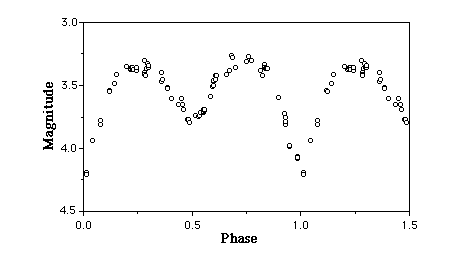
\includegraphics[scale=0.5]{LC}
\caption{Photometry of Beta Lyrae in 1992-1993}
\end{figure}

\end{enumerate}

\section*{Explanation of Light Curve}

The light curve is plotted as a consequence of the following movements of the stars in binary system.

\begin{itemize}
\item
If the stars are separated, we get lighy from both stars. Total amount of light will be indicated by the brightness on the brightness vs. time scale.
do it at home .. create figures and add phases of light curve. pages 5,6

\end{itemize}

\section{Computational Work}
The verification of Modiefied Newtonian Dynamics depends upon the Rotation Curve of the specific galaxy. The rotation curve gives us a relation between the rotational velocity and the distance of the astronomical object from teh centre. To gain the required result, I chose Andromeda Galaxy. Andromeda Galaxy is the nearest of our neighbours and its is a massive galaxy. To plot its rotation curve I was required to calculate the distances of the astronomical objects that comprise this galaxy and the mass distribution of the galaxy. Keeping the constraints of unavailability of any telescope in mind, i had to chose the technique of Image Analysis to relate the brightness to the mass distribution of the galaxy.
\subsection{Image Analysis of M31}
The image analysis is done by different techniques. It basically allows us to extract meaningful information from a digital image. There are different techniques that could be used for image analysis. Different programming languages are used for image analysis. I used Python language for this purpose. Python is a precise coding language, that allows us to write longer codes in a few lines.

The purpose of image analysis was to relate the luminous mass by using luminosity profile to the distance of each pixel from the centre. The following program was used for the whole process. The image used is just an image of a quadrant of the galaxy, and further calculations are done on the basis of an assumption of circular symmetry of the galaxy. Following is the image released by Hubble Telescope Images in $2015$ and is used for the analysis.
\begin{figure}[h!]
\centering
\includegraphics[scale=0.125]{andromeda.jpg}
\caption{Andromeda Galaxy, M31, NGC 224}
\end{figure}

\subsection{Program for Image Analysis}
The program was divided into a few parts to create a clear concept of purpose of each part. Following are the parts of the program.
\begin{enumerate}
\item \textbf{Defining the Image Dimensions}

The following code gives us the dimensions of the image being used and the spectral type of the image as the third entity.

\begin{verbatim}

andro = misc.imread('andromeda.jpg')
    (w, h,d) = andro.shape
\end{verbatim}

Output: (1918,6000,3)


\item \textbf{Calculation of the Distance of Certain Pixel from the Centre of the Galaxy}

This part defines the co-ordinates of the Origin as $x_{0}$ and $y_{0}$. This function iterates over the whole image to calaculate the distances of each pixel from the origin point by simple formula of the Pythagoras theorem.

\begin{verbatim}

x0 = 88.23
y0 =1675.78
def calc_distance(x0,y0,x,y):

    x_dist = (x - x0)
    y_dist = (y-y0)

    return  math.sqrt(x_dist*x_dist+y_dist*y_dist)

\end{verbatim}
Output:

\item \textbf{Intensity Calculation for Each Pixel}

The Intensity of each pixel is required to estimate the mass of each astronomiacal object in the galaxy, as intensity is directly proportional to the energy of the celestial object [1234].The image I used was an RGB image of the galaxy, to calculate the intensity of each pixel I had to convert it first into grayscale.This is done by fetching the RGB values of each pixel and taking square root of their squares divided by $3$. The pixel values are better to be normalized to get the results ranging from $0$ to $1$. The following part of the program explains this computation in a better way.

\begin{verbatim}

denom= math.sqrt(3)*255

def calc_gs_intensity(i):


    R = float(i[0])
    G = float(i[1])
    B = float(i[2])

    return math.sqrt(R*R+G*G+B*B)/denom


\end{verbatim}

Output:

\item \textbf{Storing the Data}

From the previously explained parts of the program, i got a large number of values. So, to use the calculated data it is necessary to create a data file, that can store maximum number of values and can again be used to plot a graph. The values from the distances and the intensity values are stored simultaneously in a single CSV (comma separated values) file.
\begin{verbatim}

with open('data.csv', 'w') as fout:

        for x in range(w):
            for y in range (h):

                r= calc_distance(x0,y0,x,y)
                i = calc_gs_intensity( andro[x,y] )

                print (r)
                print (i)

                fout.write(str(r) + "," + str(i)+ "\n")


\end{verbatim}
Output:

\item \textbf{Histogram}

Now, to analyze the mass distribution of M31, i plotted a histogram of radius versus Commulative Normalized Intensity. This gives us the mass density of the galaxy to be decreasing as we move far from the centre of the galaxy.
\begin{verbatim}
def main():

    reader = csv.reader (open('data.csv', 'rb'), delimiter=',')

    R = []
    I = []

    for row in reader:
        r= float(row[0])
        print r
        R.append( r )
        I.append( float(row[1]) )

    plt.hist(R, weights=I, bins = 100)
    plt.xlabel('radius   (pixels)    1kpc = 11.7px  ')
    plt.ylabel('Cummulative Normalized Intensity')
    plt.show()

\end{verbatim}
\begin{figure} [h]
\centering
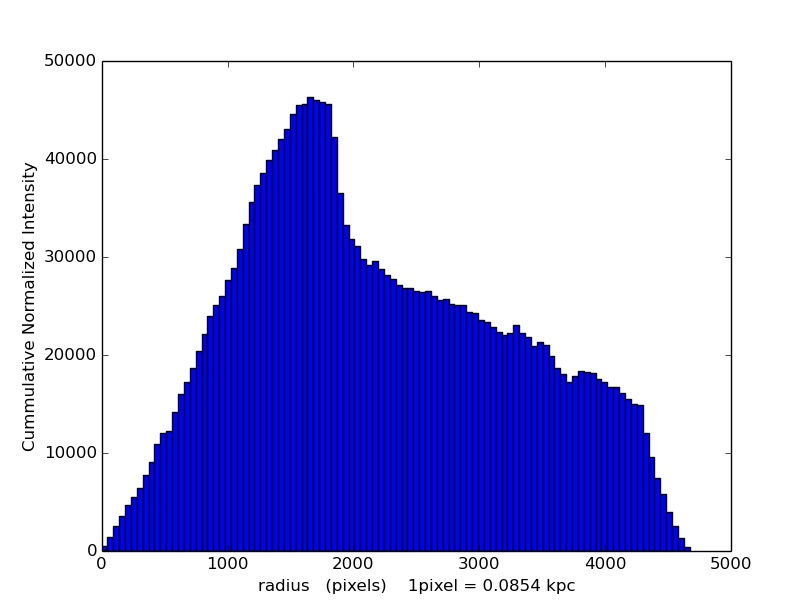
\includegraphics[scale=0.5]{histogram.jpg}
\caption{Mass Distribution of the Andromeda Galaxy }
\end{figure}


\end{enumerate}
